\section{Programovacie jazyky a kompilátory}
\indent Pri programovacích jazykoch nás zaujímajú ich vyjadrovacie schopnosti ako aj vlastnosti z hľadiska ich rozpoznania. Tieto vlasnosti sa týkajú programovania a prekladu, pričom obe je potrebné zohľadniť pri tvorbe jazyka. V dnešnej dobe sa používajú na programovanie hlavne takzvané vyššie programovacie jazyky, môžeme ich označiť ako zdrojové jazyky. Na to aby vykonávali čo používateľ naprogramoval je potrebné aby boli pretransformované do jazyka daného stroja. Spomínanú transformáciu zabezpečuje prekladač, prekladačom máme na mysli program, ktorý číta zdrojový jazyk a transformuje ho do cieľového jazyka, ktorému rozumie stroj.[1]

\subsection{Proces prekladu}
Aby bol preklad možný, musí byť zdrojový kód programu napísaný podľa určitých pravidiel, ktoré vyplývajú z jazyka. Proces prekladu je možné rodeliť na 4 hlavné časti.
\begin{itemize}
	\item lexikálna analýza
	\item syntakticka analýza
	\item spracovanie sémantiky
	\item generovanie cieľového jazyka
\end{itemize}
\indent Podrobnejšie si stručne popíšeme všetky štyri časti, ktoré majú pre nás z hľadiska prekladu najväčší zmysel.
\newline
\subsubsection{Lexikálna analýza}
	\indent Lexikálna analýza je prvou fázou kompilátora. Dopredu napísaný zdojový kód je postupne spracovávaný preprocesorom, ktorý vytvára takzvané lexémy. 
	 \newline Lexémou nazývame postupnosť alfanumerických znakov. Tieto postupnosti znakov sú následne vkladané do lexikálneho analyzátora, ktorý ma za úlohu vytvoriť zo vstupných lexém tokeny slúžiace ako vstup pre syntaktický analyzátor. 
	 \newline Tokeny sa vytvárajú na základe preddefinovaných pravidiel, ktoré sa v programovacích jazykoch definujú ako pattern. V prípade, že lexikálny analyátor nieje schopný nájsť  pattern pred danú lexému musí vyhlásiť chybu počas tokenizácie.  
	 \newline Výstupom z lexikálnej analýzy sú takzvané tokeny, ktoré tvoria vyššie jednotky jazyka ako kľúčové slová jazyka, konštanty, identifikátory, operátory a iné.
	 
	 \begin{figure}[!htbp]
	 	\centering
	 	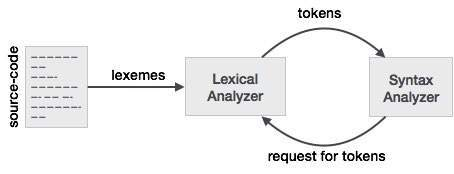
\includegraphics[width=15cm]{img/lexical_analysis.jpg}
	 	\caption{Ukážka práce lexikálneho analyzátora}
	 	\label{fig:test}
	 \end{figure}
 \newline
 
\subsubsection{Syntaktická analýza}
\indent Ďalšou fázou je syntaktická analýza. Úlohou Syntaktického analyzátora je kontrola správnosti vytvorených tokenov s uchovaním niektorých získaných informácií o štruktúre skúmanej syntaktickej jednotky. Syntaktická analýza sa radí medzi bezkontextové gramatiky. Po skoncení syntaktickej analýzy prichádza na rad sémantická analýza.

 \newline
  \newline
\begin{figure}[!htbp]
	\centering
	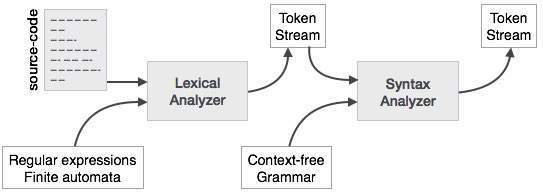
\includegraphics[width=15cm]{img/syntax_analyzer.jpg}
	\caption{Ukážka práce syntaktickeho  analyzátora}
	\label{fig:test}
\end{figure}
 \newline
 \newpage
\subsubsection{Limitácia syntaktickej analýzy}
\indent Syntaktický analyzátor ziska vstup z tokenu, ktorý vytvorí lexikálny analyzátor. Lexikálne analyzátory sú zodpovedné za validitu tokenu.Syntaktické analyzátory majú nasledovné limitácie.

\begin{itemize}
	\item nedokážu zistiť validitu tokenu
	\item nedokážu zistiť či je token používaný pred tým ako je deklarovaný
	\item nedokážu zistiť či je token používaný pred tým ako je inicializovaný
	\item nedokážu zistiť validitu operácie, ktorú token vykonáva
\end{itemize}



\subsubsection{Semantická  analýza}
\indent Sémantická analýza má za úlohu interpretovať symboly, typy, ich vzťahy.Sémantická analýza rohoduje či má syntax programy význam alebo nie.
Ako príklad zisťovania významu môžeme uviesť jednoduchú inicializáciu premennej.

\begin{lstlisting}

	int integerVariable = 6

	int secondIntegerVariable = "six"
\end{lstlisting}

Oba príklady by mali prejsť cez lexikálnu a syntaktickú analýzu. Je až na sémantickej analýze aby rozhodla o správnosti zápisu programu a v prípade nesprávneho zápisu informovala o chybe.  Hlavné úlohy sémantickej analýzy sú" :

\begin{itemize}
	\item zisťovanie dosahu definovaných tokenov takzvaný scoping
	\item kontrola typov
	\item deklaracia premenných
	\item definícia premenných
	\item viacnásobná deklarácia premenných v jedno scope
\end{itemize}

\subsubsection{Generovanie cieľového jazyka}
\indent Generovanie cieľového jazyka môžeme považovať za poslednú fázu kompilátora. V tejto fáze sa preklápa jazyk z vyššieho jazyka do strojového jazyka, ktorý úspešne prešiel cez analyzačné časti .

\subsection{Abeceda a vyhradené slová jazyka}
abeceda jazyka, popis ake pismena-slova rozpoznava, ake su vyhradene slova jazyka a bla bla


\subsection{Procedúry a algoritmy}
procedúra - konečná postupnosť inštrukcií, ktorá sa dá vykonať mechanicky.

\section{Operačné systémy}

\subsection{Windows}
\indent Microsoft Windows uviedol svoje prvé operačné systémy v roku 1985 ako nadstavbu MS DOS. Jeho popularita rýchlo rástla až vyvrcholila dominantným postavením na trhu v osobných počítačoch. V roku 1993 začal vydávať špecializované operačné systémy pre servery, ktoré prinášali novú funkcionalitu pre počítače používané ako servery. Pre účely automatizácie sa na Windows serveroch používajú hlavne powershell scripty, písane v rovnomennom jazyku powershell.
\newline
\subsection{MacOs}
\indent  Mac tiež ponúka serverovú verziu svojho operačného systému pod názvom OS X Server, ktorý začal písať svoju históriu v roku 2001, avšak neteší sa takej obľube ako Windows, unix alebo linux server. Skriptovacím jazykom pre OS X server nieje špecifický jazyk, je možné vybrať si z Pythonu, JavaSriptu, Perl, AppleScriptu, Swiftu alebo napríklad Ruby. Každý jazyk prináša určité plusy, ale zároven mínusy čo je však najpodstatnejšie nie je tam štandardizovaný skriptovací jazyk.
\newline
\subsection{Unix}
\indent Patrí medzi prvé operačné systémy pre servery, ktorých vývoj začal v roku 1970 v priebehu rokov vzniklo nespočetné množstvo nových verzií Unixu. Unixové servery sa tešil veľkej obľube hlavne v minulosti momentálne sú na ústupe hlavne kvoli vyšším nákladom na ich zaobstaranie a prevázku. Pre účely unixu sa vytvoril shell script, oľúbený scriptovací jazyk, ktorý sa v rôznych obmenách teší veľkej obľube medzi administrátormi a automatizačnými programátormi.
\newline
\subsection{Linux}
\indent  Prvé vydanie Linux  bolo 17. septembra 1991, bol rozšírený na najviac platforiem a momentálne sa pýši tým, že je jediný používany operačný systém na TOP 500 superpoťétačoch9(mainframoch) Skriptovací jazyk shell script.
\newline
\section{ Skriptovacie jazyky}
\indent S príchodom počítačov, hlavne serverov, sa programátori zaujímali o automatizáciu procesov, ktoré na danom stoji bolo spočiatku potrebné spúšťať manuálne.
Vačšina serverov bežalo na Unixových distribúciách.

\subsection{Shell}
\indent
Je skriptovacím jazykom pre unixové distribúcie. Počas rokov prešiel roznymi zmenami a rozšíreniami. Verzie shellu su: sh, csh, ksh,tcsh, bash. Bash sa momentálne teši najväčšej obľube no zsh je verzia shellu, ktorá má najviac rôznych rozšírení funkcionality ako aj veľa priaznivcov medzi developermi. V nasledujúcich častiach všeobecne zhodnotíme jednotlivé výhody resp. nevýhody tohoto skriptovacieho jazyka.

\subsubsection{Výhody}
\begin{itemize}
\item automatizácia často opakujúcich sa úloh
\item dokáže zbiehať zloťité zloťené príkazy ako jednoriadkový príkaz  - tzv. reťazenie príkazov
\item ľahký na používanie
\item výborné manuálové stránky
\item ak hovoríme o shell scripte je portabilný naprieč platformami linuxu-unixu
\item jednoduché plánovanie automatických úloh
\newline
\end{itemize}
\subsubsection{Nevýhody}
\begin{itemize}
\item asi najväčšou nevýhodou je ze natívne nefunguje pod windowsom, existuju iba rozne emulátory a 3rd tooly, ktoré sprostredkujú jeho funkcionalitu.
\item pomalé vykonávanie príkazov pri porovnaní s inými programovacími jazykmi
\item nový proces pre skoro každý spustený príkaz
\item zložitejší na pamatanie si rôznych prepínačov, ktoré dané príkazy podporujú
\item nejednotnosť prepínočov(hoc to by asi ani nešlo)
\end{itemize}
\subsubsection{Popis a zhodnotenie jazyka}
\noindent
Shell script je obľúbeným scriptovacím jazykom, vhodným na automatizovanie každodenných operácií. Je jedným z najpoužívanejších skriptovacích jazykou vôbec, nakoľko všetky linuxove, unixové servery využívajú práve tento jazyk ako svoj primárny.
Medzi jeho silné stránky patrí jednoduchá manipulácia s crontable, pomocou ktorej vie admin jednoducho planovať beh procesov.
Avšak syntax jazyka sa učí tažšie nakoľko používa rôzne prepínače, ktoré novému používateľovi nemusia byť sprvu jasné.
V tabuľke uvádzame príklad prepínačov pre if, tiež je vhodné poznamenať, že shell script používa hranaté zátvorky namiesto okrúhlych na aké sme zvyknutý z väčšiny programovacích jazykov. If ponúka aj ďalšie prepínače no zhodnotili sme, že pre ilustráciu budú postačovať aj ukázané.
Najvačsia nevýhoda je, že ani shell script nieje jazyk, ktorý by bol multiplatformový a teda ak by sme mali prostredie, kde servery bežia na rôznych operačných systémoch, potrebujeme poznať ďalší jazyk, ktorým docielime rovnaké alebo aspoň podobné výsledky.
\newline
\begin{table}[h!]
	\centering
	\begin{tabular}{| c | c | }
		\hline
		String Comparison	&Description\\
		\hline
		Str1 = Str2	& Returns true if the strings are equal\\ 
		\hline
		Str1 != Str2 &	Returns true if the strings are not equal\\ 
		\hline
		-n Str1	 &R eturns true if the string is not null\\ 
		\hline
		-z Str1	& Returns true if the string is null\\
		\hline
		\hline
		Numeric Comparison	&Description\\
		\hline
		expr1 -eq expr2	& Returns true if the expressions are equal\\
		\hline
		expr1 -ne expr2	& Returns true if the expressions are not equal\\
		\hline
		expr1 -gt expr2	& Returns true if expr1 is greater than expr2\\
		\hline
		expr1 -ge expr2	& Returns true if expr1 is greater than or equal to expr2\\
		\hline
		expr1 -lt expr2	& Returns true if expr1 is less than expr2\\
		\hline
		expr1 -le expr2	& Returns true if expr1 is less than or equal to expr2\\
		\hline
		! expr1	& Negates the result of the expression\\
	    \hline
	\end{tabular}
\caption{Ukážka prepínačov v podmienkovom výraze if}
\label{table:1}
\end{table}
\newpage

\subsection{Powershel/Classic command line}
\indent
Je zakladnym skriptovacim jazykom pre windows distribucie.
Powershell je nasledovni classic shellu.  
Jeho vyhody a nevyhody si popiseme v nasledujujucich castiach.

\subsubsection{Výhody}
rychlost
podpora napriec linux unix 
ludia ho poznaju
dokumentacia
\subsubsection{Nevýhody}
asi najvacsou nevyhodou je ze nativne nefunguje pod windowsom, existuju iba rozne emulatory a 3rd tooly, ktore sprostredkuju jeho funkcionalitu.

\section{Analýza existujucich riešeni}
\indent
Existuje mnozstvo emulatorov a 3rd toolov, ktore sprostredkuvaju funkcionality bashu do windowsu.

Zoznam najlepsich rieseni najdenych na internet:
-cmder- vyuziva ConEmu s vylepseniami clink
-ConEmu
-Babun - poskytuje bash + zsh
-MobaXterm
- ZOC Terminal - ZOC is a professional SSH/telnet client and terminal emulator. With its impressive list of emulations and features, it is a snap to access hosts and mainframes via secure shell, telnet, serial cable, modem/isdn and other methods of communication.
- Console2-  facilitates the running of CMD, PowerShell, Cygwin, PuTTY, etc.g.


\section{Architektúra aplikácie}
DSL - domain specific language
\subsection{Pouzite navrhove vzory}
Aby sme zaručili rozšíriteľnosť, manažovateľnosť a ďalšie zásady dobrého softwéru bolo potrebné zvoliť vhodnú arhitektúru, ktorú popisujú použité návrhové vzory.
\subsubsection{Command - príkaz}
\indent Command pattern je známy behaviorálny návrhový vzor, používa sa najmä na menežovanie algoritmov, vzťahov a zodpovednosti medzi objektami. 
Cieľom vzoru je zapúzdriť požiadavku(request) ako objekt tým pádom parametrizovať klienta s rôznymi požiadavkami a zabezpečiť operáciu spať.
\begin{figure}[!htbp]
	\centering
	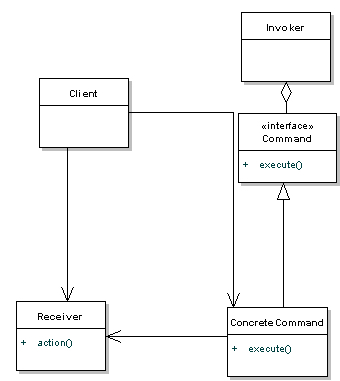
\includegraphics[width=10cm]{img/command_pattern_class.jpg}
	\caption{Class diagram Command návrhového vzoru}
	\label{fig:test}
\end{figure}
\newline
Command vzor deklaruje interface pre všetky budúce commandy a zároveň execute() metódu, ktorú s vypýta Receiver commandu aby splnil požadovanú operáciu.
Receiver je objekt, ktorý vie ako požadovanú operáciu splniť. Invoker pozná command a pomocou implementovanej execute() metódy dokáže vyvolať požadovanú operáciu.
Klient potrebuje implemenotvaž ConcreteCommand a nastavit Receiver pre command. ConcreteCommand definuje spojenie medzi action a receiver. Keď Invoker zavolá execute() metódu na ConcreteCommand spustí tým jednu alebo viac akcií, ktoré budú bežať pomocou Receivera.

Pre lepšie pochopenie je proces zobrazený aj na sekvenčnom diagrame.
\begin{figure}[!htbp]
	\centering
	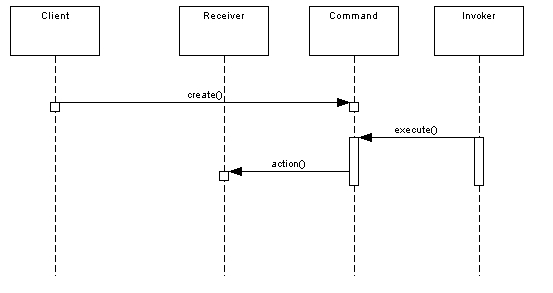
\includegraphics[width=10cm]{img/command_seq.jpg}
	\caption{Sekvenčný diagram Command návrhového vzoru}
	\label{fig:test}
\end{figure}
\newline

\subsubsection{Factory - továreň}
\indent Factory návrhový vzor patrí do sekcie vytváracích vzorov, pomocou tohoto vzoru budeme schopný vytvárať objekty bez toho aby sme prezradili logiku ich vytvárania klientovi.
Diagram návrhového vzoru je mozné vidieť na nasledujúcom obrázku.
\begin{figure}[!htbp]
	\centering
	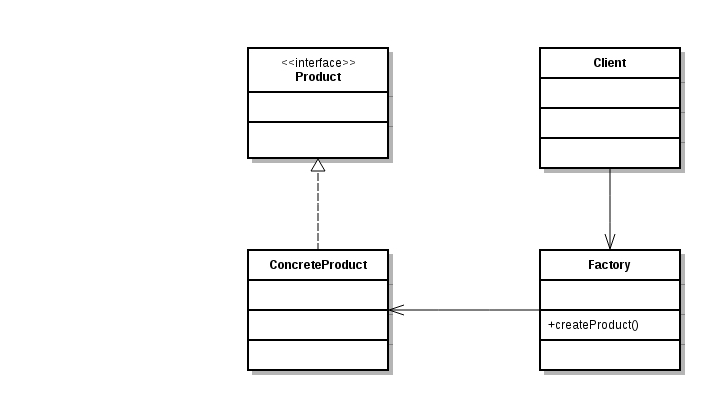
\includegraphics[width=10cm]{img/factory_design_pattern.jpg}
	\caption{Class diagram Factory návrhového vzoru}
	\label{fig:test}
\end{figure}
\newline

\subsubsection{Interpreter}
mozno pouzijem
\subsection{Komponenty aplikácie}
\indent Aplikacia zalozena na plugin systeme.
Popisat scoping
Vytvaranie commandov

\section{Zhodnotenie výsledkov}
Zatiaľ sa toho nespravilo hodne ale verím, že sa to tu cele zaplní.